\chapter{Podatkovne zbirke Svetovne Banke}

Pri diplomski nalogi smo se osredoto"cili na dva programska vmesnika za dostop 
podatkov Svetovne banke, to sta ``ClimateAPI'' s katerim dostopamo do 
podatkovne zbirke meteorolo"skih meritev in ``IndicatorAPI'' s katerim dostopamo do 
zbirke podatkov raznih indikatorjev stopenj razvoja dr"zav.
Za uporabo podatkovne zbirke Svetovne banke smo se odlo"cili, ker zdru"zuje in na
enovit na"cin predstavi podatke iz ve"cih razli"cnih virov. Podatkovni viri za 
indikatorje stopnje razvoja dr"zav so:
\begin{itemize}  
  \item Svetovni indikatorji razvoja~\cite{world_dev_ind} % World Development Indicators, 
  \item Globalni finan"cni razvoj~\cite{glob_fin_dev}
  \item Afri"ski indikatorji razvoja~\cite{africa_dev_ind}
  \item Poslovanje~\cite{doing_buseness},
  \item Podjetni"ske raziskave~\cite{ent_surveys}, 
  \item Razvojni cilji~\cite{mil_dev_goals}, 
  \item Statistike izobra"zevanja~\cite{edu_stat}, 
  \item Statistike spolov~\cite{gen_stat},
  \item Statistike zdravja in prehranjevanja~\cite{health_pop_stat},
  \item Rezultati meritev IDA~\cite{ida_res_mes_sys}.
\end{itemize}  

Podatkovni vir zbirke podnebnih meritev pa je osnovan na podatkih oddelka
za podnebne raziskave (ang.\ Climatic Research Unit)~\cite{climate_data}.

Svetovna banka omogo"ca dostop do podatkov preko programskega vmesnika REST, ki
ponuja veliko mo"znosti za iskanje in presejanje rezultatov. Pri vsaki 
poizvedbi REST lahko dolo"cimo "zeljeno obliko odgovora. Za poizvedbe o 
informacijah indikatorjev sta na voljo obliki XML in JSON. Programski vmesnik 
meteorolo"skih meritev pa ponuja samo obliko JSON. Za konsistentnost in la"zjo
berljivost smo na obeh programskih vmesnikih uporabili obliko JSON. To na
programskem vmesniku indikatorjev dosezemo take da nastavimo parameter GET
\verb|format| na vrednost \verb|json|. 


\section{Podatki indikatorjev razvoja dr"zav}
\label{sec:podatki_ind_razvoja}



Programski vmesnik indikatorjev razvoja dr"zav Svetovne banke omogo"ca dostop
do podatkov preko 16.000 raznih indikatorjev. Podatki indikatorjev so merjeni
mese"cnem, "cetrtletnem ali letnem intervalu. Za"cetek meritev podatkov
posameznega indikatorja je odvisna od vira podatkov. Najstare"si podatki segajo
do leta 1960. Poleg podatkov indikatorjev nam ta programski vmesnik omogo"ca 
tudi dostop do ve"cine metapodatkov s katerimi lahko presejamo in natan"cneje
dolo"cimo na"so poizvedbo. Seznami metapodatkov so:
\begin{itemize}
\item viri podatkov in njihovi opisi (ang.\ Catalog Source Queries
	\fnurl{http://api.worldbank.org/sources?format=json}),
\item seznam dr"zav, skupin dr"zav in regij z identifikatorji (ang.\ Country Queries
	\fnurl{http://api.worldbank.org/countries?format=json}),
\item razdelitev vi"sin dohodkov z identifikatorji (ang.\ Income Level Queries
	\fnurl{http://api.worldbank.org/incomeLevels?format=json}),
\item seznam indikatorjev (ang.\ Indicator Queries
  \fnurl{http://api.worldbank.org/indicators?format=json}),
\item seznam tipov posojil (ang.\ Lending Type Queries
	\fnurl{http://api.worldbank.org/lendingTypes?format=json}),
\item seznam tem (ang.\ Topics \fnurl{http://api.worldbank.org/topics}).
\end{itemize}

Za pridobitev podatkov indikatorjev potrebujemo metapodatke o indikatorjih in
dr"zavah. Primere teh metapodatkov si bomo podrobneje pogledali v nadaljevanju.

Ker je mogo"ce z eno poizvedbo dostopati do velike koli"cine podatkov, ima
programski vmesnik za dostop do podatkov indikatorjev implementirano
ostranjevanje, s katerim je omejeno "stevilo podatkov ki jih lahko dobimo z eno
poizvedbo. Tako so podatki razdeljeni na skupine ki jih imenujemo strani.

Vsi odgovori na veljavne poizvedbe po podatkih in metapodatkih, ki so na voljo
s programskim vmesnikom indikatorjev razvoja, imajo enako osnovno obliko. 
Poizvedbe vra"cajo seznam z dvema elementoma, kjer je ima prvi element 
informacije o koli"cini podatkov in trenutnem izboru podatkov, drugi element 
pa vsebuje seznam izbranih podatkov (Primer \ref{basic_response}). Privzeta
vrednost "stevila elementov na stran je $50$, kar lahko spremenimo tako da
poizvedbi nastavimo parameter GET \verb|per_page| na poljubno vrednost. "Ce
"zelimo pridobiti podatke z ve"cih strani, moramo za vsako stran poslati novo
poizvedbo v kateri podamo "zeljeno stran s parametrom GET \verb|page|, . 
Veljavne poizvedbe, s sitom ki ne vra"ca nobenih podatkov, imajo vrednost 
drugega elementa osnovnega seznama \verb|null|.
Za neveljavne poizvedbe, pa programski vmesnik vraca seznam z enim elementom,
ki vsebuje podatke o napaki poizvedbe (Primer \ref{error_response}).


\begin{snippet}
\begin{center}
\begin{lstlisting}
[
    {
        "page": 1,
        "pages": 137,
        "per_page": "50",
        "total": 6831
    },
    [
        <podatki>,
        ...
    ]
]
\end{lstlisting}
\end{center}
\caption{Osnovna oblika odgovora programskega vmesnika Svetovne banke, za
veljavno poizvedbo indikatorjev.} 
\label{basic_response}
\end{snippet} 


\begin{snippet}
\begin{center}
\begin{lstlisting}
[
    {
        "message": [
            {
                "id": "120",
                "key": "Parameter 'country' has an invalid value",
                "value": "The provided parameter value is not valid"
            }
        ]
    }
]
\end{lstlisting}
\end{center}
\caption{Osnovna oblika odgovora programskega vmesnika Svetovne banke, za
neveljavne poizvedbe.}
\label{error_response}
\end{snippet} 


\subsection{Opis seznama indikatorjev}

Programski vmesnik Svetovne banke za indikatorje razvoja nam ponuja seznam 
vseh indikatorjev z imeni, opisi, kodami in drugimi metapodatki 
(Primer \ref{indicator_response}). Programski vmesnik nam tudi omogo"ca dostop
do podatkov posameznega indikatorja dolocenega s kodo in presejanje seznama 
indikatorjev glede na vir podatkov \ref{indicator_queries}. V nasem programu
smo uporabili le poizvedbo za celotn seznam indikatorjev, da smo omogocili 
iskanje in presejanje po vseh poljih indikatorjev.

\begin{snippet}
\begin{center}
\begin{lstlisting}
http://api.worldbank.org/indicators?format=json
http://api.worldbank.org/indicators?format=json&source=5
http://api.worldbank.org/indicators/A10i?format=json
\end{lstlisting}
\end{center}
\caption{Primeri poizvedb po seznamu indikatorjev.
1) seznam vseh indikatorjev, 2) seznam indikatorjev glede na vir podatkov,
3) podatki indikatorja ``A10i''}
\label{indicator_queries}
\end{snippet} 


\begin{snippet}
\begin{center}
\begin{lstlisting}
{
    "id": "1.0.HCount.2.5usd",
    "name": "Poverty Headcount (\$2.50 a day)",
    "source": {
        "id": "37",
        "value": "LAC Equity Lab"
    },
    "sourceNote": "The poverty headcount index measures the 
                   proportion of the population with daily per 
                   capita income (in  2005 PPP) below the poverty
                   line.",
    "sourceOrganization": "LAC Equity Lab tabulations of SEDLAC 
                           (CEDLAS and the World Bank).",
    "topics": [
        {
            "id": "11",
            "value": "Poverty "
        }
    ]
}
\end{lstlisting}
\end{center}
\caption{Podatki indikatorja 
% TODO
% Ali moram ime indikatorja oznaciti (naprimer velika zacetnica)
% > Podatki indikatorja Stopnja rev...
stopnja rev"s"cine pri dohodku 2,5 dolarja na dan.}
\label{indicator_response}
\end{snippet} 

\subsection{Opis seznama dr"zav}

Seznam dr"zav na programskem vmesniku Svetovne banke vsebuje podatke o imenih, 
opisih, ISO-3166-1 alpha kodah, regijah in druge metapodatke 
(Primer \ref{country_response}). Programski
vmesnik nam tudi omogo"ca presejanje seznama dr"zav po kodi dr"zave, regiji,
visini dohodka, in tipu posojil (Premer \ref{country_queries})

% \begin{description}
% \item [id] koda dr"zave, regije ali skupine dr"zav,
% \item [region] regija,
% \item [incomeLevel] vi"sina dohodka,
% \item [lendingType] tipov posojil. % TODO preveri prevod!
% \end{description}

\begin{snippet}
\begin{center}
\begin{lstlisting}
http://api.worldbank.org/countries?format=json
http://api.worldbank.org/countries/svn?format=json
http://api.worldbank.org/countries?format=json&incomeLevel=HIC&region=ECS
\end{lstlisting}
\end{center}
\caption{Primeri poizvedb po seznamu dr"zav.
1) seznam vseh dr"zav, 2) podatki ene dr"zave,
3) seznam dr"zav v Evropi in Osrednji Aziji, z visoko vi"sino dohodka.}
\label{country_queries}
\end{snippet} 

Ta seznam ne vsebuje zgolj samo dr"zav, ampak tudi regije in skupine dr"zav, 
zdru"zenih glede na razli"cne kriterije (vi"sine dohodka, velikost, stopnja
razvoja). Poleg tega zgornji seznam vsebuje tudi nekatere izjeme kot je trenutno
Kosovo. V nadaljevanju bomo za vse na"stete tipe lokacijskih podatkov
uporabljali besedo ``dr"zave''. 

\begin{snippet}
\begin{center}
\begin{lstlisting}
{
    "id": "ABW",
    "iso2Code": "AW",
    "name": "Aruba",
    "region": {
        "id": "LCN",
        "value": "Latin America & Caribbean "
    },
    "adminregion": {
        "id": "",
        "value": ""
    },
    "incomeLevel": {
        "id": "HIC",
        "value": "High income"
    },
    "lendingType": {
        "id": "LNX",
        "value": "Not classified"
    },
    "capitalCity": "Oranjestad",
    "longitude": "-70.0167",
    "latitude": "12.5167"
},
\end{lstlisting}
\end{center}
\caption[some]{Izsek podatkov veljavne poizvedbe dr"zav.}
\label{country_response}
\end{snippet} 


\subsection{Dostop do podatkov indikatorjev}

Za dostop do podatkov posameznega indikatorja, potrebujemo kodo
indikatorja s seznama vseh indikatorjev in kodo ene ali ve"cih dr"zav. Namesto
kode ene ali ve"cih dr"zav lahko uporabimo tudi klju"cno besedo ``all'', ki
ozna"cuje vse kode dr"zav. Pri ve"cjih koli"cinah podatkov, lahko z dodatnimi
parametri dolo"cimo "stevilo podatkov na stran, in "zeljeno stran podatkov.
Primer \ref{indicator_dataset_request} prikazuje osnovno obliko poizvedbe,
kjer so:
\begin{description}
\item [country] s podpi"cjem lo"cen seznam kod izbranih dr"zav, ki jih 
	  preberemo iz polja ``id'' ali ``iso2Code'', ki sta prikazana v Primeru 
    \ref{country_response}, ali pa klju"cna beseda ``all'',
\item [indicator\_id] polje ``id'' indikatorja ki je prikazano v Primeru 
    \ref{indicator_response}.
\item [parametri] Dodatni parametri GET 
\end{description}
Za poizvedbe do podatkov indikatorjev so poleg osnovnih parametrov GET 
\verb|per_page|, \verb|page| in \verb|format|, opisanih v poglavju 
\ref{sec:podatki_ind_razvoja}, na voljo tudi dodatni parametri za presejanje
rezultatov poizvedbe:
\begin{description}  
\item [MRV] Stevilska vrednost, ki dolo"ci maksimalno "stevilo zadnjih meritev,
    ki jih programski vmesnik vrne. Ko uporabljamo polje \verb|mrv| bo 
    programski vmesnik izpustil ni"celne vrednosti za obdobja v katerih ni
    meritev.
\item [gapfill] Zastavica \verb|'y'| ali \verb|'n'| za manjkajo"ce vrednosti meritev.
    Vrednost \verb|'y'| kombinaciji z poljem \verb|mrv| poskrbi da programski 
    vmesnik ne izpusti nobenega "casovnega intervala.
\item [date] Polje obilke \verb|'leto'| ali \verb|'leto:leto'| ki omeji rezultate poizvedbe
    na dolo"ceno leto ali interval med dolo"cenimi leti. 
\end{description}


\begin{snippet}
\begin{center}
\begin{lstlisting}
http://api.worldbank.org/en/countries/<country>/indicators/<indicator_id>?<parametri>
\end{lstlisting}
\end{center}
\caption{Osnovna oblika poizvedbe za podatke enega indikatorja.}
\label{indicator_dataset_request}
\end{snippet} 

% http://api.worldbank.org/countries/svn/indicators/SL.TLF.ACTI.FE.ZS?format=json
% http://api.worldbank.org/countries/svn;usa/indicators/SL.TLF.ACTI.FE.ZS?format=json
% http://api.worldbank.org/countries/all/indicators/SL.TLF.ACTI.FE.ZS?format=json

Privzeta vrednost za koli"cino podatkov na stran \verb|per_page| je 50. 
Zgornja meja pa ni strogo dolo"cena, vendar je odvisna od velikosti odgovora. 
Ugotovili smo, da se zanesljivost programskega vmesnika manj"sa z ve"cjo 
koli"cino podatkov na stran. V na"sem programu smo se omejili na 1000 podatkov
na stran, kar se je izkazalo za uporabno razmerje med hitrostjo in 
zanesljivostjo programskega vmesnika. Privzeto bo programski vmesnik vrnil 
podatke za vse "casovne vrednosti. V odgovoru API-ja dobimo seznam objektov 
(Primer \ref{dataset_response}) z datumom, indikatorjem, dr"zavo in vrednostjo.

\begin{snippet}
\begin{center}
\begin{lstlisting}
{
    "indicator": {
        "id": "SP.POP.TOTL",
        "value": "Population, total"
    },
    "country": {
        "id": "IL",
        "value": "Israel"
    },
    "value": "6289000",
    "decimal": "0",
    "date": "2000"
}
\end{lstlisting}
\end{center}
\caption{Podatki za indikator SP.POP.TOTL (populacija dr"zave) za Izrael leta
2000.}
\label{dataset_response}
\end{snippet} 

Slabost programskega vmesnika indikatorjev Svetovne banke je v tem, da ne
moremo z eno poizvedbo dostopati do podatkov ve"cih indikatorjev hkrati.

\section{Podatki podnebnih meritev}

Programski vmesnik Svetovne banke za podnebne podatke omogo"ca dostop do 
podatkov napovednih modelov in zgodovinskih meritev meteorolo"skih postaj. V tej 
diplomski nalogi smo se odlo"cili uporabiti samo podatke zgodovinskih meritev, 
saj si s temi podatki lahko uporabnik programa Orange sam sestavi svoje 
napovedne modele.

Za razliko od uporabe programskega vmesnika indikatorjev, lahko pri tem
programskem vmesniku uporabljamo veljavne ISO 3166-1 alpha-2 ali ISO 3166-1 
alpha-3 kode dr"zav, ali pa "stevilski identifikator vodoto"cnega 
obmo"cja.

Ta programski vmesnik nam omogo"ca dostop do podatkov o povpre"cnih 
temperaturah in padavinah v "casovnih obdobjih enega leta, desetletja ali pa 
nam omogo"ca dostop do mese"cnih povpre"cij skozi vsa leta meritev.


\subsection{Dostop do podatkov podnebnih meritev}

Za dostop do podnebnih podatkov preko programskega vmesnika Svetovne banke,
potrebujemo ISO-3166-1 alpha3 kodo dr"zave, ali "stevilski identifikator
vodoto"cnega obmo"cja (Slika \ref{climate_data_api_basins}). Programski vmesnik
nam omogo"ca dostop do meritev povprecnih koli"cin padavin in temperatur za 
letno ali desetleno obdobje. Poleg letnega in desetletnega obdobja pa nam 
programski vmensik ponuja tudi povprecno kolicino padavin in temperatur za 
posamezne mesece skozi vsa leta meritev. Obliko poizvedbe prikazuje primer 
\ref{climate_dataset_request}, kjer je:
\begin{description}
\item [loc\_type] vrsta identifikatorja obmo"cja (``basin'' za vodotocno obmo"cje, 
  ``country'' za dr"zave),
\item [data\_type] vrsta meritev (``pr'' za padavine, ``tas'' za temperature),
\item [interval] vrsta meritvenega obdobja (``month'' za mese"cno, ``year'' za letno in
  ``decade'' za desetletno),
\item [location] koda dr"zave ali stevilski identifikator vodoto"cnega obmo"cja.
\end{description}
Za razliko od programskega vmesnika indikatorjev, nam programskem vmesniku
podnebnih meritev z eno poizvedbo omogoca dostop do podatkov le za eno dr"zavo.
To pomeni da je koli"cina podatkov dovolj omejena da nam programski vmesnki,
vedno vrne vse podatke brez ostranjevanja, kot prikazuje primer 
\ref{climate_dataset_response},


\begin{figure}
\begin{center}
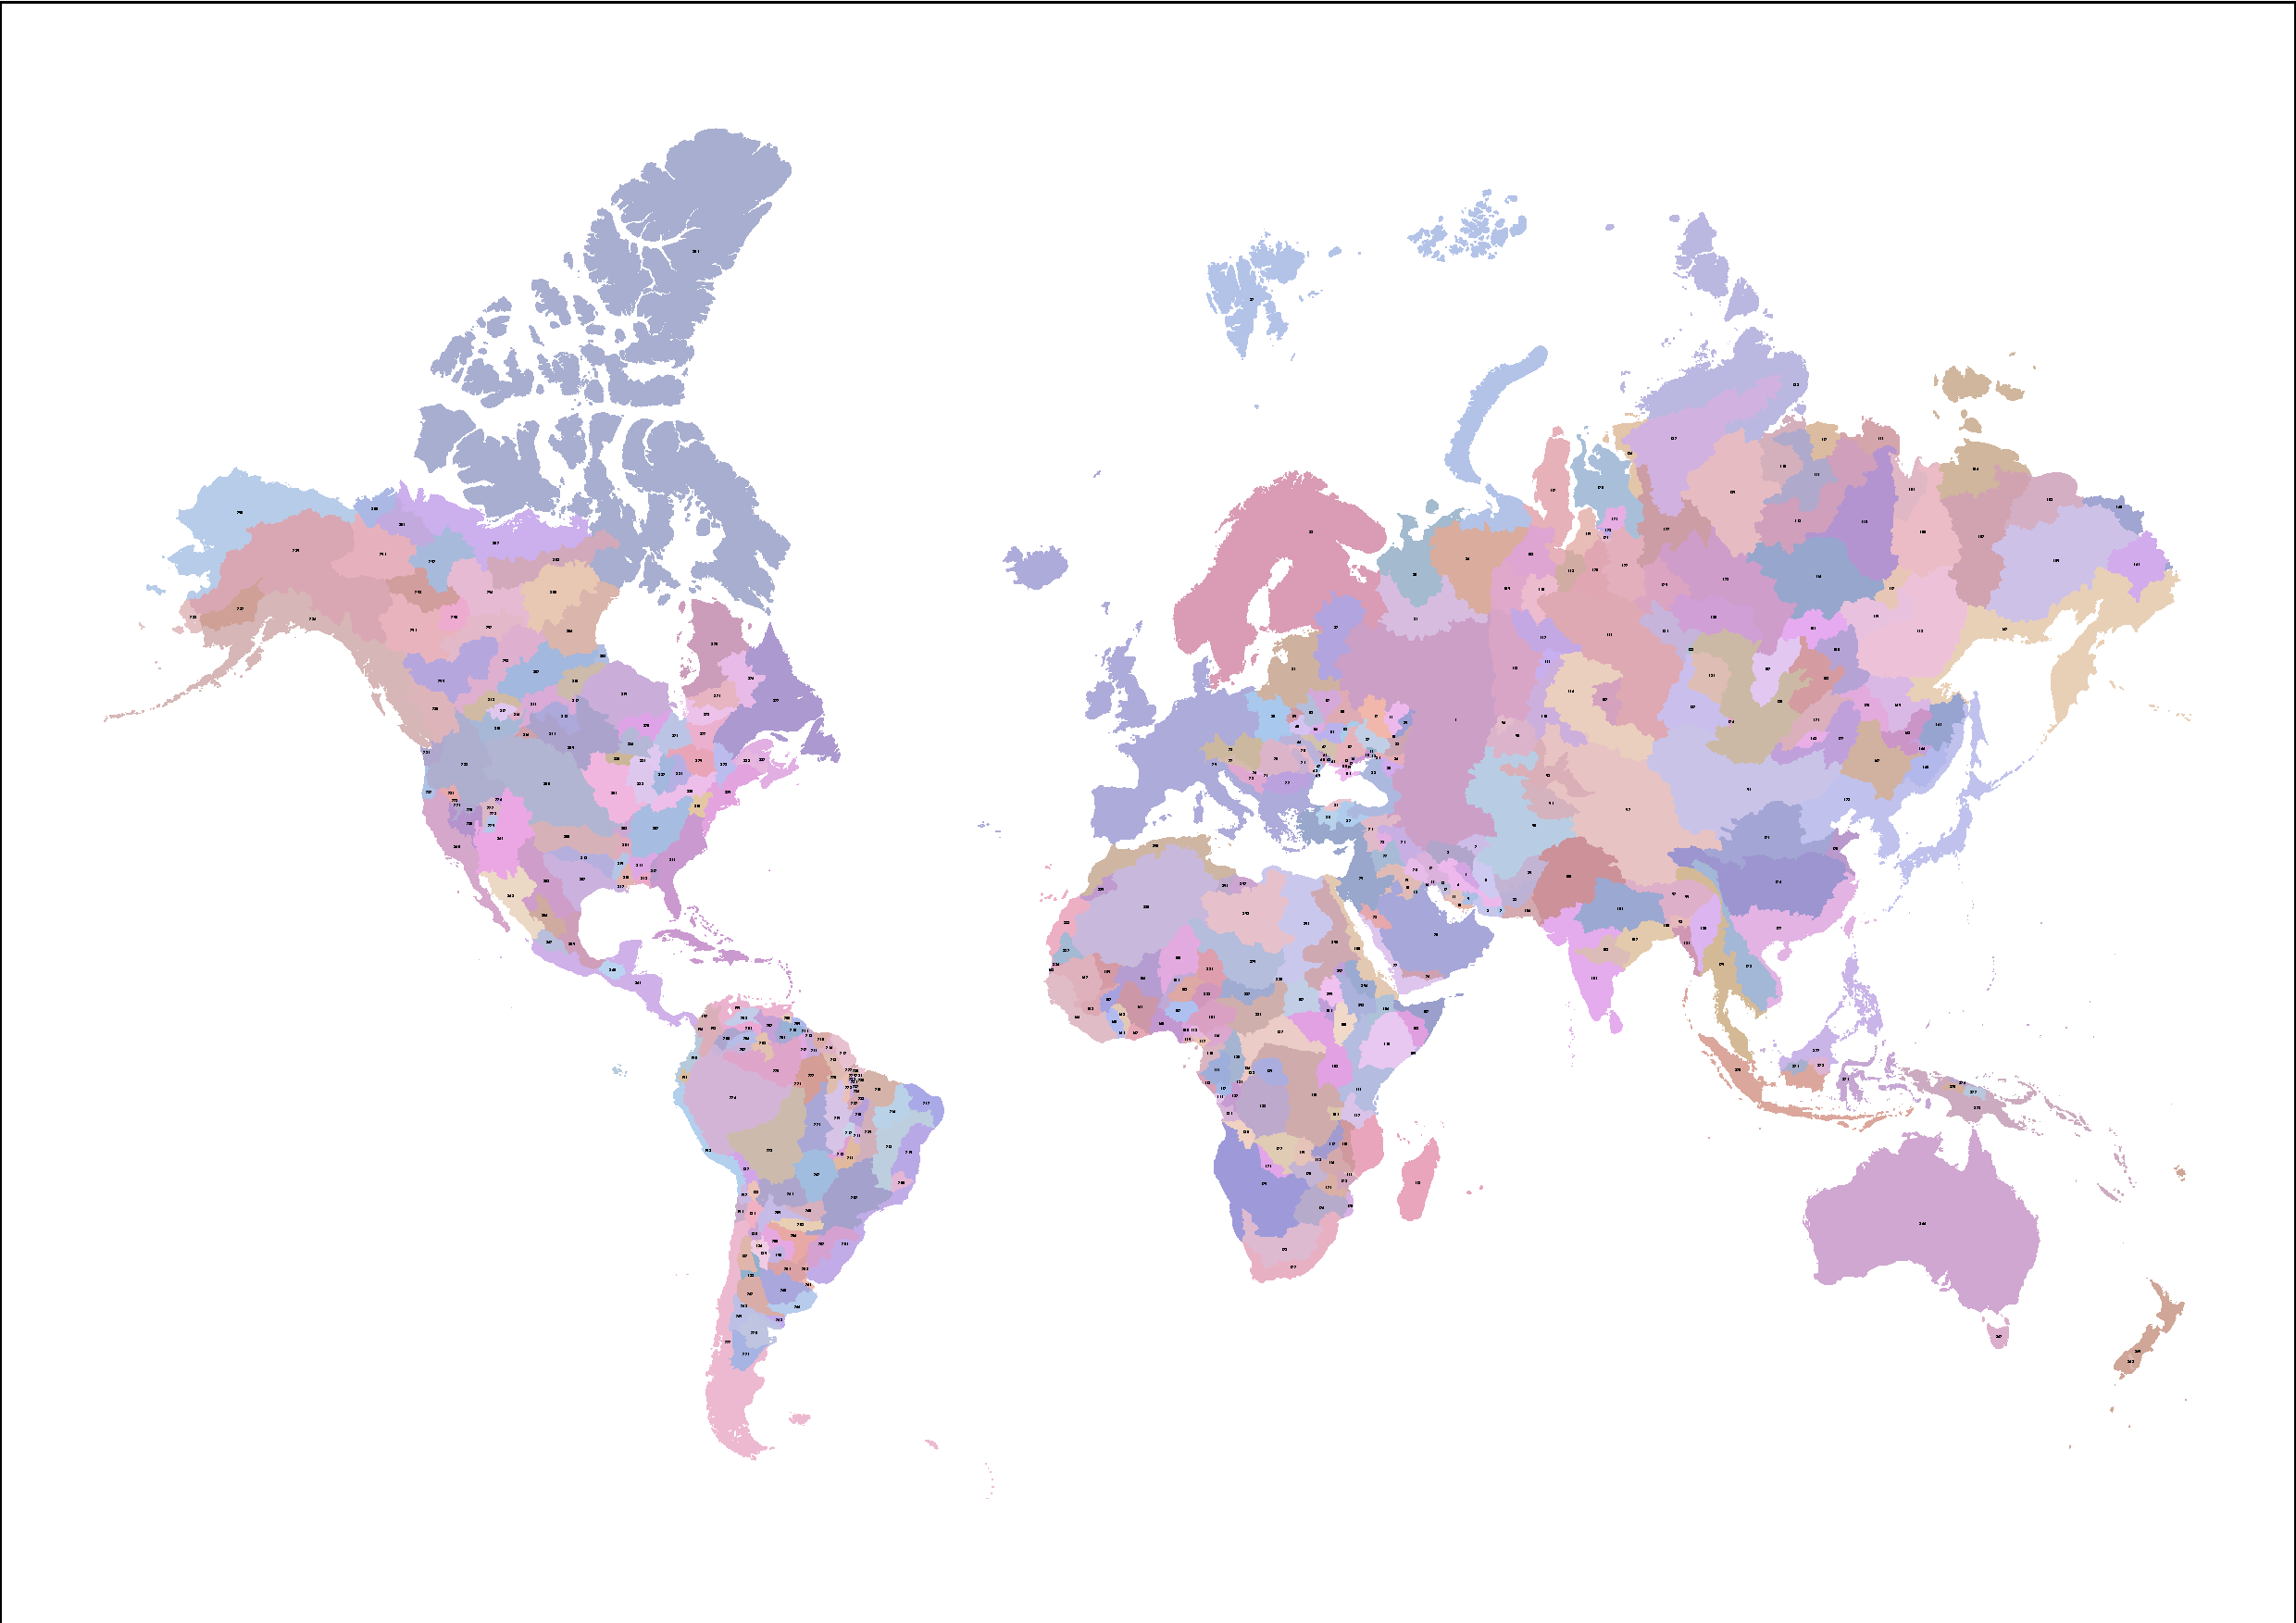
\includegraphics[width=12cm]{pic/climate_data_api_basins.pdf}
\end{center}
\caption{Prikaz vodoto"cnih obmo"cij sveta.}
\label{climate_data_api_basins}
\end{figure} 


\begin{snippet}
\begin{center}
\begin{lstlisting}
http://climatedataapi.worldbank.org/climateweb/rest/v1/<loc_type>/cru/<data_type>/<interval>/<location>
\end{lstlisting}
\end{center}
\caption{Osnovna oblika poizvedbe za podnebne podatke.}
\label{climate_dataset_request}
\end{snippet} 


\begin{snippet}
\begin{center}
\begin{lstlisting}
[
    {
        "month": 0,
        "data": 68.93643
    },
    {
        "month": 1,
        "data": 64.23069
    },
    {
        "month": 2,
        "data": 81.098724
    },
    ...
]
\end{lstlisting}
\end{center}
\caption{Primer odgovora za poizvedbo koli"cine padavin v posameznih mesecih v 
  Sloveniji.}
\label{climate_dataset_response}
\end{snippet} 











\section{Te"zave pri uporabi programskih vmesnikov Svetovne banke}


Programski vmesniki Svetovne banke zajema podatke razli"cnih virov, zato je
te"sko zagotoviti pravilnost in konsistentnost podatkov. Poleg tega pa se 
programski vmesnik in spletna stran z dokumentacijo ob"casno spremenita, kar
povzro"ca "se dodatne te"zave pri uporabi. Nekatere te"zave, ki smo jih opazili
so:
\begin{itemize}  
\item nekaterim delom dokumentacije se je med izdelavo te diplomske naloge
  spremenil spletni naslov, tako da do tistit delov sedaj nimamo ve"c dostopa,
\item polje za datum v odgovoru je opisano, vendar ni dokumentirano, kak"sne so
    vse mo"zne vrednosti (nekaj primerov nedokumentiranih vrednosti:
    ``last known value'' ``2001 - 2015'' ``2040''),
\item delovanje sita z razli"cnimi kombinaciji polj \verb|mrv|, \verb|gapfill|
  in \verb|date| ni ustrezno opisano,
\item v odgovoru poizvedbe po podatkih indikatorjev, ponekod manjkajo vrednosti
  kot so koda dr"zave, ime dr"zave ali ime indikatorja.
\item zgornja meja "stevila izbranih lokacij na 250 ni navedena in napaka 
  ki jo programski vmesnik vrne ni dokumentirana,
\item nemogo"ce je ugotoviti pogostost vzor"cenja indikatorja (frequency), .
\end{itemize}  







